% Gemini-based Academic Presentation Poster (1-Page A0 Landscape)
% Conforming strictly to Boğaziçi University CMPE 492 Poster Presentation Standards
% Dimensions: ISO A0 Landscape (1189 mm x 841 mm)
% Project: Çok Dilli Eğitim Teknolojisi (ASR -> LLM Terminoloji & Pedagojik DAG)
% Institution: Boğaziçi Üniversitesi Bilgisayar Mühendisliği Bölümü

\documentclass[final]{beamer}

% ====================
% Packages
% ====================

\usepackage[size=a0, orientation=landscape, scale=1.2]{beamerposter}
\usetheme{gemini}
\usecolortheme{gemini}

\usepackage{graphicx}
\usepackage{booktabs}
\usepackage{tikz}
\usepackage{pgfplots}
\pgfplotsset{compat=1.17}
\usepackage{amsmath,amssymb}
\usepackage{tabularx}
\usepackage{colortbl}
\usepackage{caption}

% Column width configuration for 4 columns on A0 Landscape (Width 1189mm, Height 841mm)
\newlength{\sepwidth}
\newlength{\colwidth}
\setlength{\sepwidth}{0.012\paperwidth}
\setlength{\colwidth}{0.233\paperwidth}

\newcommand{\separatorcolumn}{\begin{column}{\sepwidth}\end{column}}

% ====================
% Title & Metadata
% ====================

\title{\textbf{EduTerm AI:} Çok Dilli Eğitim Konuşmalarından ASR ve LLM Tabanlı \\ Terminoloji Çıkarma ve Pedagojik Bilgi Çizgesi (DAG) Değerlendirmesi}

\author{\textbf{Ali Ayhan Günder}$^1$, \textbf{Berat Enes Dadak}$^2$, \textbf{Efe Batur Giritli}$^2$, \textbf{Yekta Said Can}$^2$ \samelineand \textbf{Tez Danışmanı:} Prof. Dr. Fatih Alagöz$^1$}

\institute{$^1$Boğaziçi Üniversitesi Bilgisayar Mühendisliği Bölümü \samelineand $^2$Tatilsepeti Ar-Ge Merkezi}

% Official Boğaziçi University Emblem in top-right header
\headerlogo{
\includegraphics[height=5.0cm,keepaspectratio]{img/boun_official_logo.png}}

\begin{document}

\footercontent{
  \begin{columns}[c]
    \begin{column}{0.56\linewidth}
      \textbf{İLETİŞİM:} Ali Ayhan Günder \samelineand \textbf{Kurum:} Boğaziçi Üniversitesi Bilgisayar Mühendisliği Bölümü \\
      \textbf{E-posta:} gunderaliayhan@gmail.com \samelineand \textbf{Proje Web:} EduTerm AI Studio (Whisper + Qwen 2.5 7B LoRA + DAG + RAG)
    \end{column}
    \begin{column}{0.42\linewidth}
      \raggedleft
      \textbf{Boğaziçi Üniversitesi Bilgisayar Mühendisliği Bölümü} \\
      CMPE 492 Lisans Bitirme Projesi 2026 $\cdot$ Boğaziçi HPC (A40 48GB) $\cdot$ Millî EVREN (H200) $\cdot$ A0 Şablon
    \end{column}
  \end{columns}
}

\begin{frame}[t]
\begin{columns}[t,totalwidth=0.98\paperwidth]

% =========================================================================
% KOLON 1: Problem, Hedef (AIM), Akustik Pipeline ve Mel-Spektrogram
% =========================================================================
\separatorcolumn

\begin{column}{\colwidth}

  \begin{block}{GİRİŞ VE MOTİVASYON (PROBLEM)}
    \begin{itemize}
      \item \textbf{Teknik Jargon Bariyeri:} Üniversite ders videolarında dinleyicilerin heterojen ön bilgisi bilişsel aşırı yüke (\emph{cognitive overload}) yol açmaktadır.
      \item \textbf{Bireyselleştirme Engeli:} Birebir özel ders desteği başarıyı \textbf{2 standart sapma (Bloom 2-sigma)} artırabilir; ancak insan eğitmen desteği kitlesel ölçekte sürdürülemez.
      \item \textbf{Otomasyon İhtiyacı:} ASR ve LLM entegrasyonu, video akışından anlık terim yakalayıp pedagojik iskele (\emph{scaffolding}) oluşturma potansiyeline sahiptir.
    \end{itemize}
  \end{block}

  \vskip-0.3ex
  \begin{exampleblock}{HEDEF VE KAPSAM (AIM)}
    \textbf{Temel Amaç:} Çok dilli eğitim konuşmalarında (TR/EN) Whisper, Qwen3-ASR ve Nemotron mimarileri ile açık ağırlıklı yerel LLM'leri (Qwen 2.5/3.5) ve Millî EVREN YZ Platformu'nu (H200); 12 disiplini kapsayan 40 videoluk (10.1 sa üstveri; 4.6 sa doğrulanmış 16/40) korpus envanteri ve ölçülen 7 derslik ASR/terim deney kümesinde doğruluk, hız, bellek ve terim yakalama ($F_1$) eksenlerinde değerlendirmektir.
  \end{exampleblock}

  \vskip-0.3ex
  \begin{block}{AKUSTİK PİPELİNE VE MİMARİ}
    \begin{itemize}
      \item 16 kHz Mono ses, 30s pencereler ve Whisper \texttt{sequential\_generate()} moduyla işlenir (\%95 depolama tasarrufu).
    \end{itemize}

    \vskip0.3ex
    \centering
    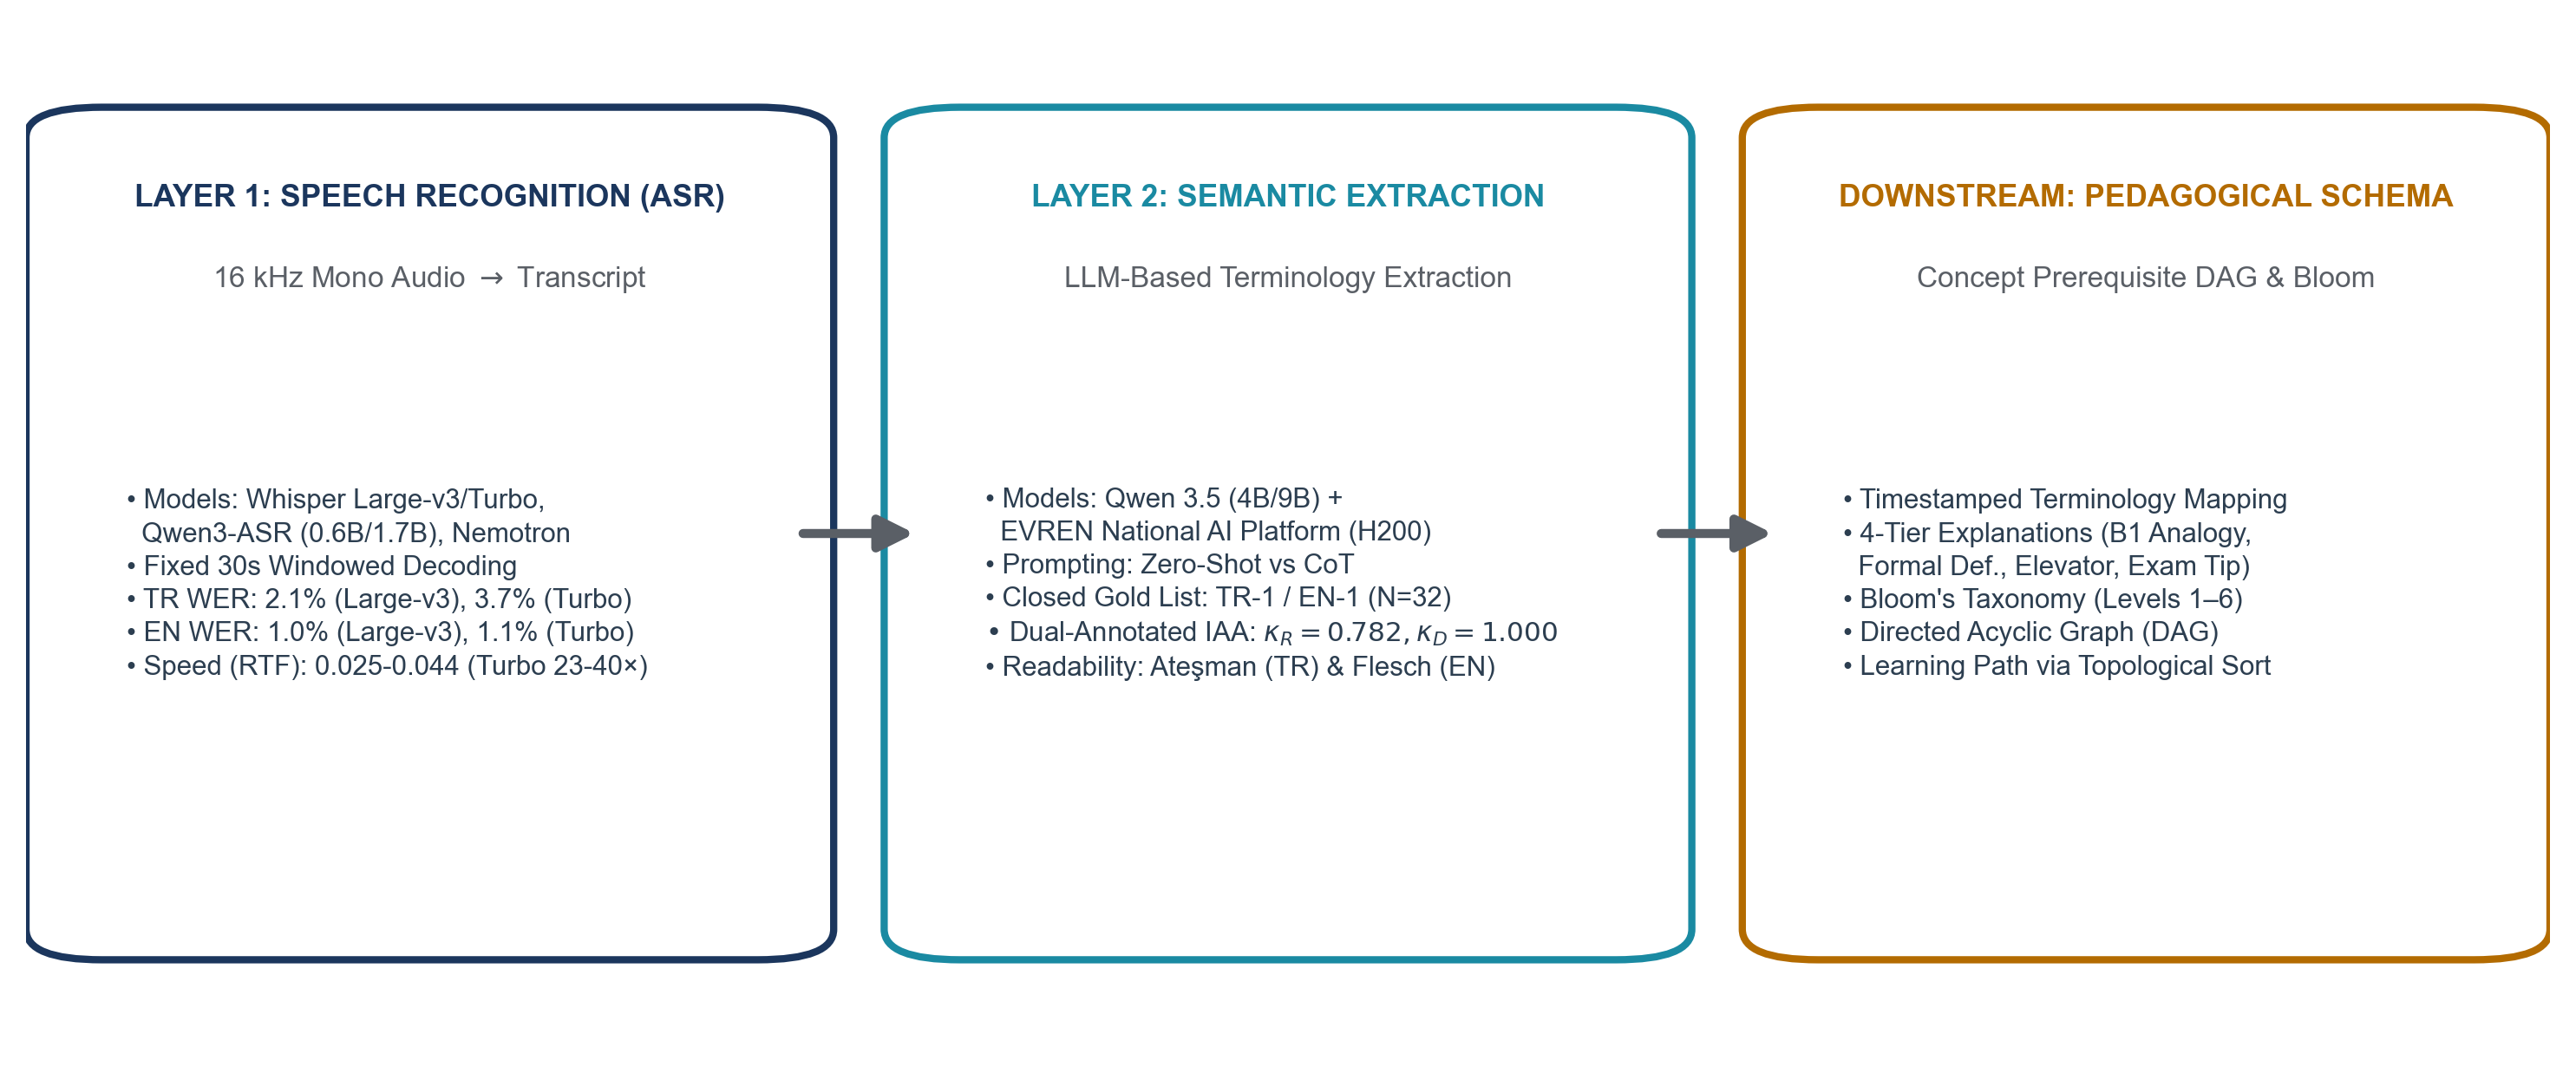
\includegraphics[width=\linewidth,height=6.5cm,keepaspectratio]{img/pipeline_architecture.png}
    \captionof{figure}{Şekil 1: Uçtan Uca Çok Katmanlı Mimari Pipeline.}

    \vskip0.3ex
    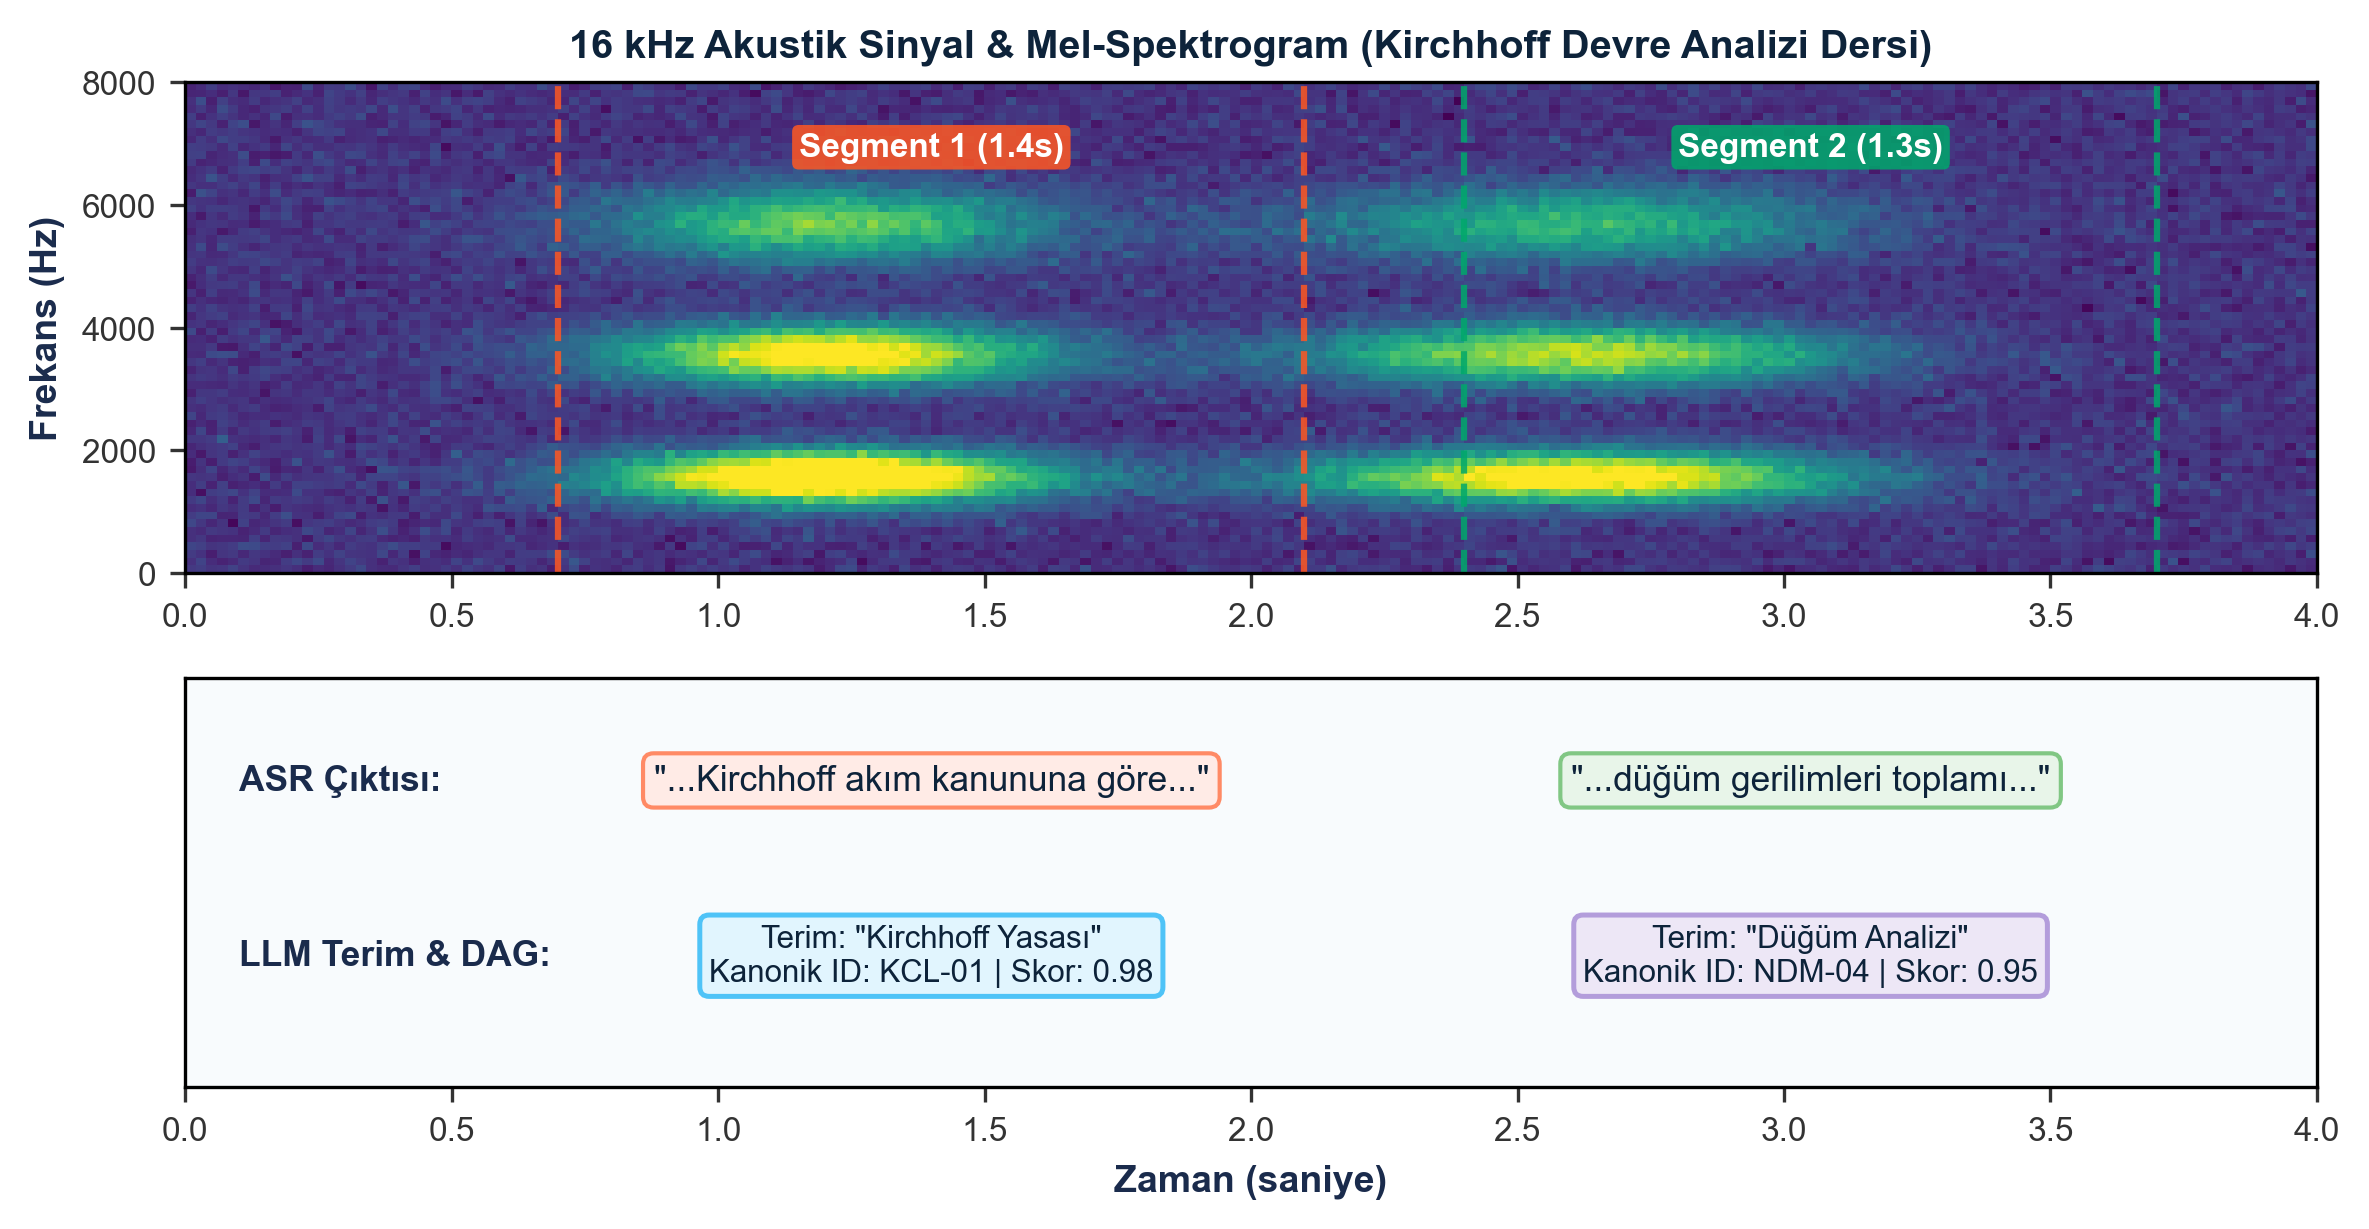
\includegraphics[width=\linewidth,height=6.2cm,keepaspectratio]{img/acoustic_spectrogram_extraction.png}
    \captionof{figure}{Şekil 2: Akustik Mel-Spektrogram ve Zaman Damgalı Terim Çıkarımı.}
  \end{block}

\end{column}

% =========================================================================
% KOLON 2: 40 Videoluk Envanter ve 7 Derslik ASR Kıyaslaması (WER)
% =========================================================================
\separatorcolumn

\begin{column}{\colwidth}

  \begin{block}{40 VİDEOLUK EĞİTİM KORPUS ENVANTERİ}
    \begin{itemize}
      \item \textbf{12 Disiplinlik Envanter:} Mühendislik, Tıp, Fizik, Matematik, Sosyal Bilimler ve kurumsal eğitimler (KVKK, İSG). 10.1 sa kaynak üstverisi (diskte doğrulanmış 16/40 klipte 4.6 sa); ASR başarım ölçümleri 7 derslik doğrulanmış test kümesindedir.
      \item \textbf{Çift Değerlendirici:} İki bağımsız araştırmacı ile $N=115$ terim altın etiketlenmiştir ($\kappa_R = 0.782$ ilgililik, $\kappa_D = 1.000$ tanım doğruluğu).
    \end{itemize}

    \vskip0.2ex
    \centering
    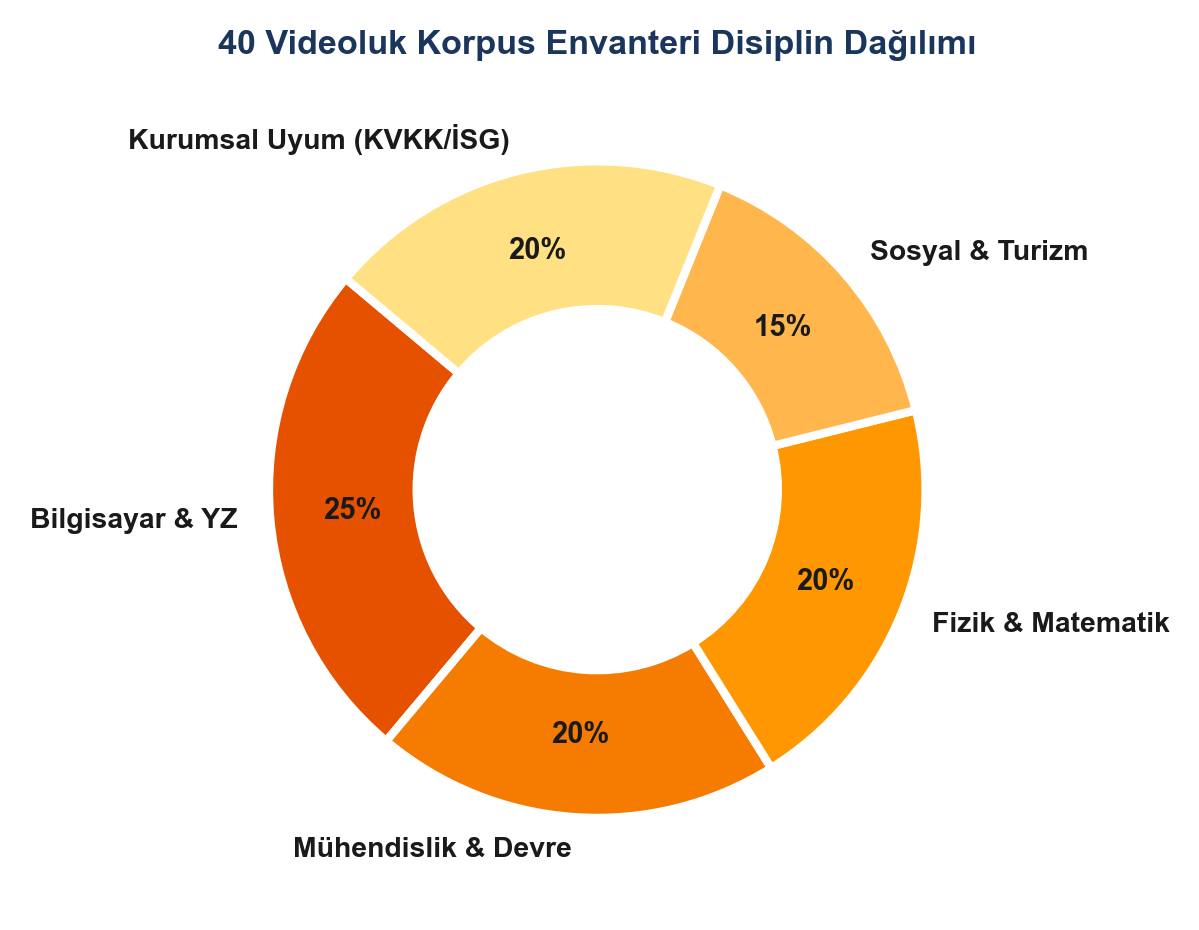
\includegraphics[width=0.88\linewidth,height=7.2cm,keepaspectratio]{img/chart_a_donut.png}
    \captionof{figure}{Şekil 3: Korpus Disiplin Dağılımı (Mühendislik, Temel Bilimler, Sosyal).}
  \end{block}

  \vskip-0.3ex
  \begin{block}{ÇOK DİLLİ ASR MODEL KIYASLAMASI (WER)}
    \centering
    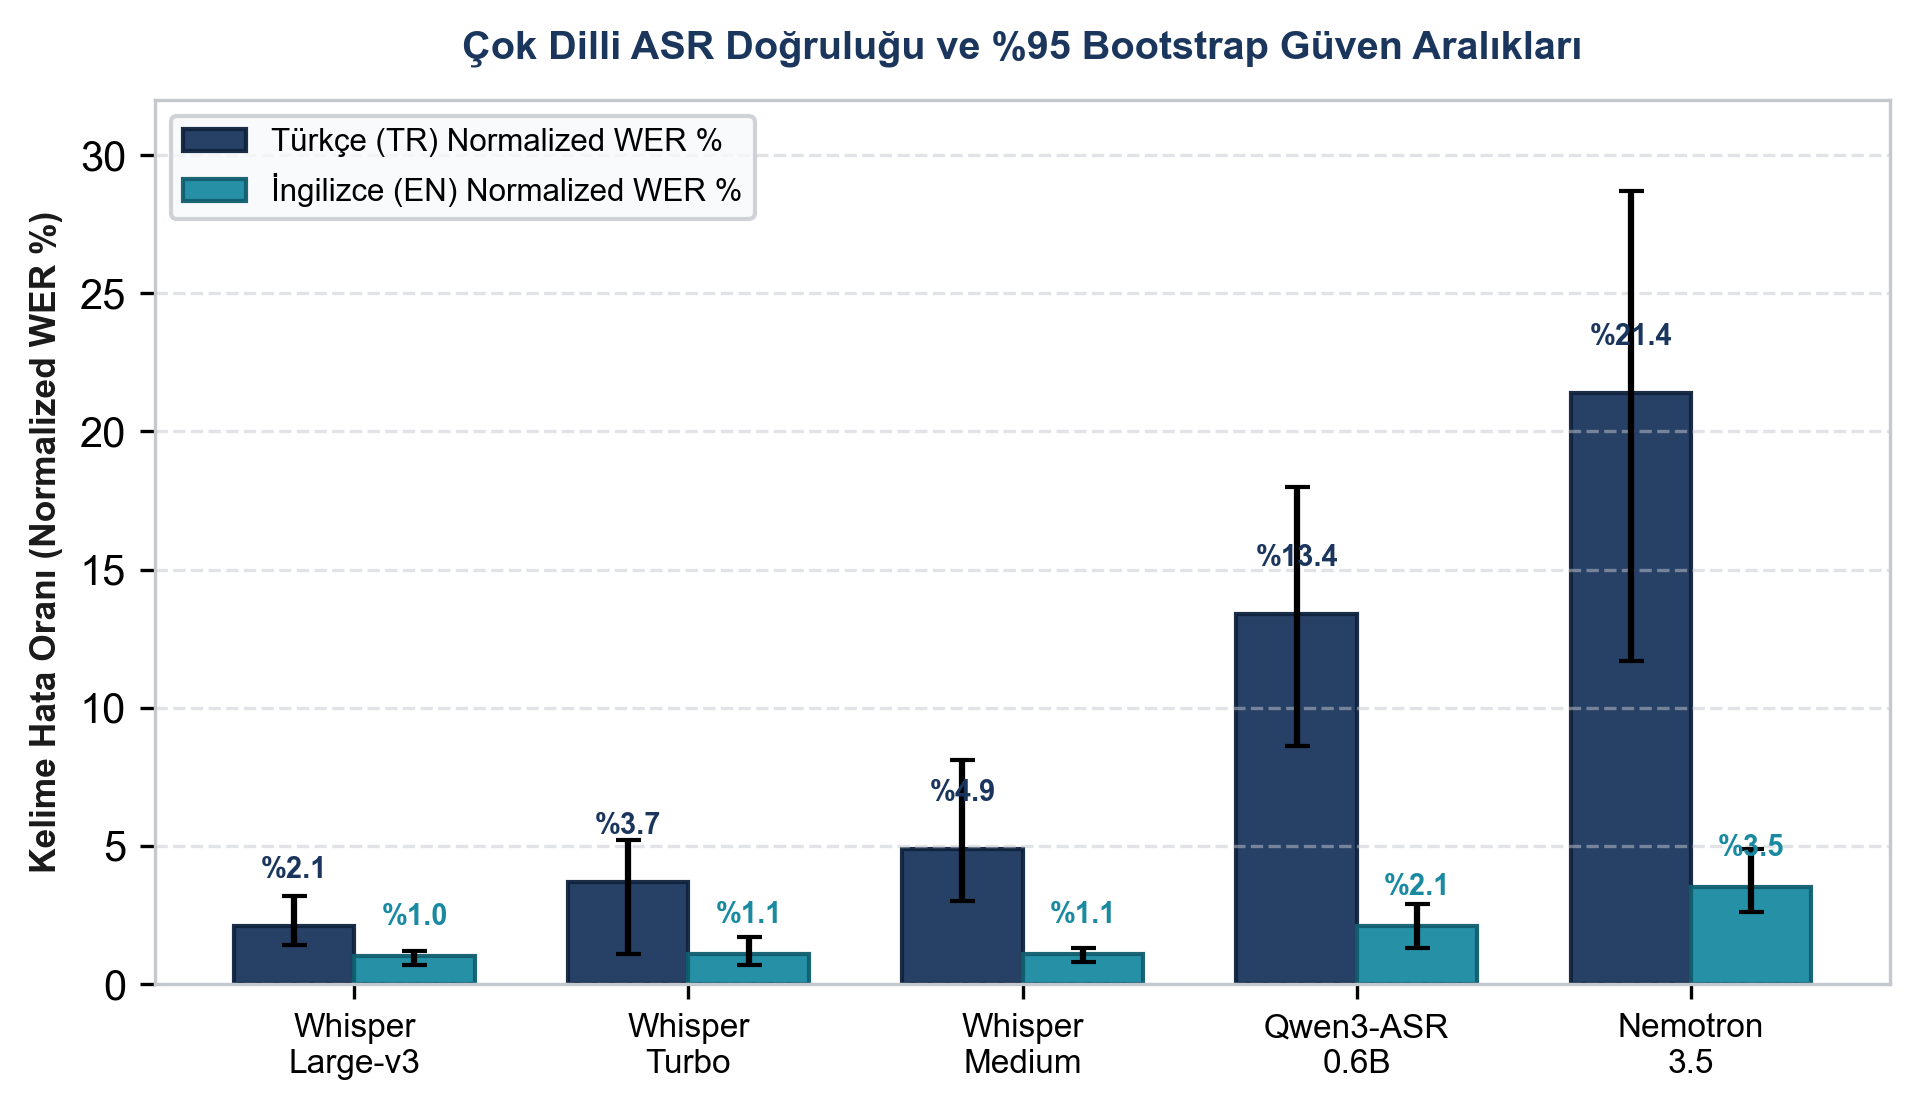
\includegraphics[width=\linewidth,height=7.0cm,keepaspectratio]{img/asr_benchmark_chart.png}
    \captionof{figure}{Şekil 4: Çok Dilli ASR Normalize WER ve \%95 GA ($B=10\,000$).}

    \begin{itemize}
      \item \textbf{Whisper Large-v3 Lider:} TR'de \%2.1, EN'de \%1.0 WER ile en yüksek doğruluğu elde etmiştir.
      \item \textbf{Whisper Turbo Hız Avantajı:} RTF 0.025--0.044 ile gerçek zamanın 23--40 katı hız sağlamıştır.
      \item \textbf{VAD Kısıtı:} Enerji tabanlı VAD teknik terim uçlarını kestiğinden WER \%2.1'den \%4.1'e kötüleşmiştir.
    \end{itemize}
  \end{block}

  \vskip-0.3ex
  \begin{block}{TABLO 1: MİLLÎ EVREN (H200), BOĞAZİÇİ HPC (A40) VE YEREL GPU}
    \small
    \begin{tabularx}{\linewidth}{>{\raggedright\arraybackslash}X c c c}
      \toprule
      \rowcolor{deepnavy}
      \textcolor{white}{\textbf{Model / Altyapı}} & \textcolor{white}{\textbf{TR Süre}} & \textcolor{white}{\textbf{EN Süre}} & \textcolor{white}{\textbf{Ortam}} \\
      \midrule
      \textbf{EVREN Qwen 3.8F} & \textbf{6.11 s} & \textbf{4.23 s} & Millî Bulut (H200) \\
      \textbf{Boğaziçi HPC (A40)} & \textbf{15.28 s} & \textbf{12.45 s} & 7B LoRA (48GB A40) \\
      \textbf{EVREN DeepSeek} & 27.68 s & 24.12 s & Yüksek Hacim \\
      \textbf{Qwen 3.5-4B (Local)} & 39.80 s & 34.20 s & RTX 5060 (4-bit) \\
      \textbf{Qwen 3.5-9B (Local)} & 513.19 s & 322.29 s & CPU Offload \\
      \bottomrule
    \end{tabularx}
  \end{block}

\end{column}

% =========================================================================
% KOLON 3: Dikey LoRA, Hibrit RAG ve Çapraz Katman Hata Yayılımı
% =========================================================================
\separatorcolumn

\begin{column}{\colwidth}

  \begin{block}{BOĞAZİÇİ HPC (NVIDIA A40) 7B LORA EĞİTİMİ}
    \begin{itemize}
      \item \textbf{A40 Kümesi Eğitimi:} Boğaziçi HPC sunucusunda (\texttt{ultramarine}, İş ID \texttt{33580}), \texttt{Qwen2.5-7B-Instruct} modeline $r=16, \alpha=32$ LoRA ince ayarı yapılmıştır.
      \item \textbf{Eğitim Hızı ve Bellek:} 3 epoch eğitim sadece \textbf{13.67 saniyede} tamamlanmış; tepe VRAM \textbf{27.84 GB} olarak ölçülmüştür (yerel 8GB GPU'da anında OOM).
      \item \textbf{Görülmemiş Disiplinlerde Artış:} CS/BST benchmarkında terim yakalama ($Recall$) \%0.0'dan \textbf{\%33.3}'e yükselmiş; pedagojik açıklama sadeliği (Ateşman) negatiften pozitif B1 bandına (\textbf{+25.7}) sıçramıştır.
    \end{itemize}

    \vskip0.2ex
    \centering
    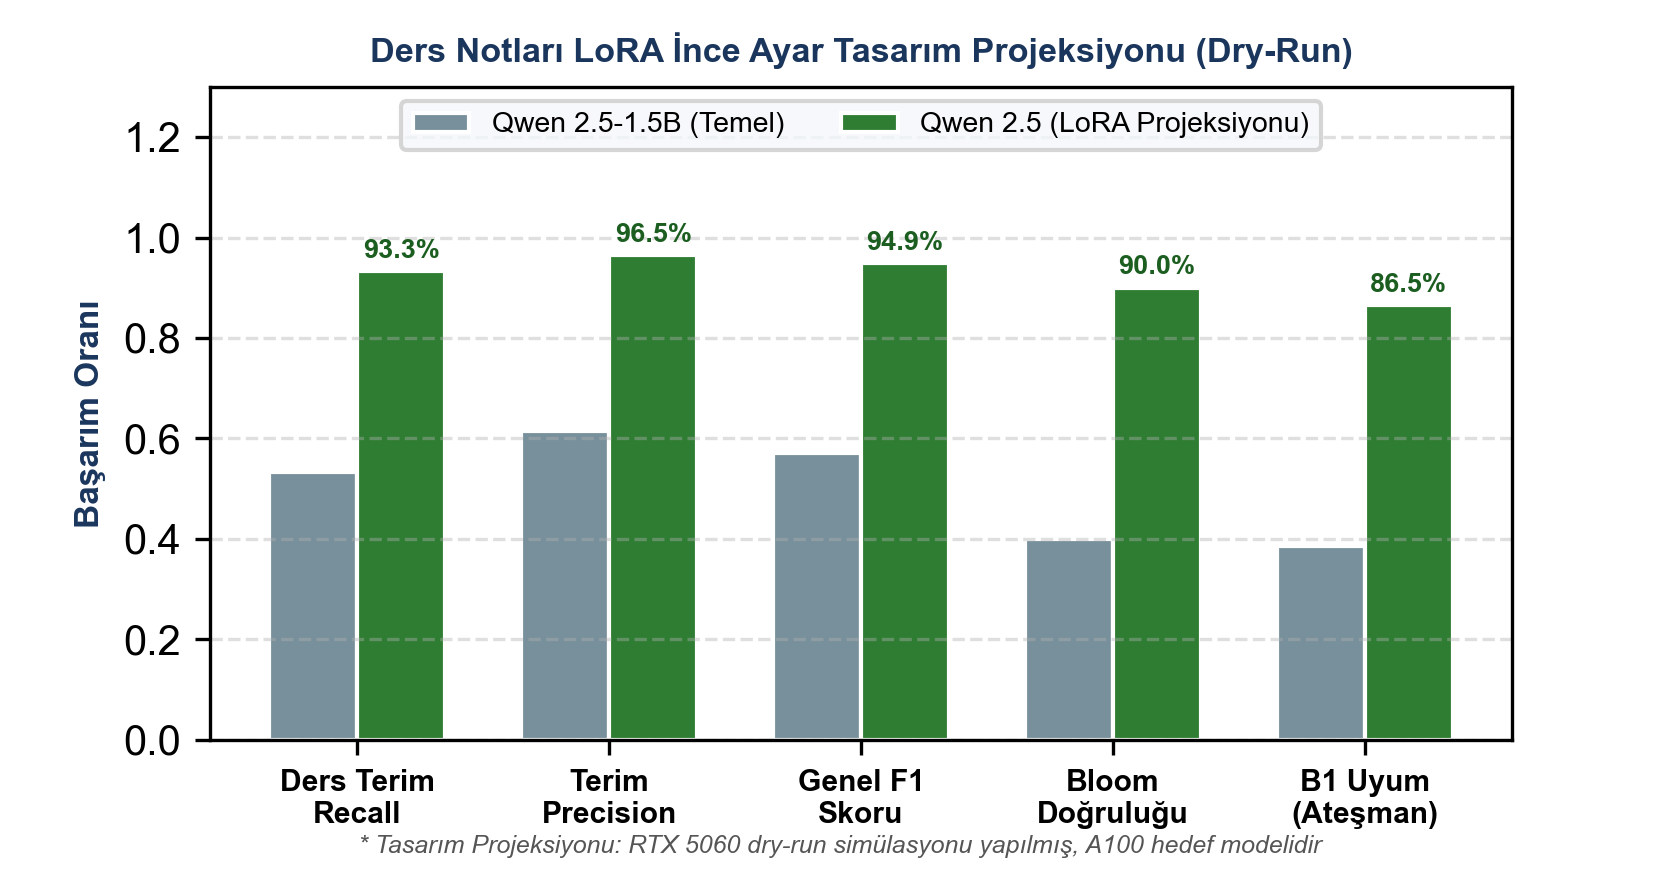
\includegraphics[width=\linewidth,height=6.2cm,keepaspectratio]{img/finetune_gain_chart.png}
    \captionof{figure}{Şekil 5: Qwen 2.5-7B LoRA İnce Ayar ve Okunabilirlik Kazanımı.}
  \end{block}

  \vskip-0.3ex
  \begin{block}{HİBRİT RAG VE ÖNKOŞUL GRAFI}
    \centering
    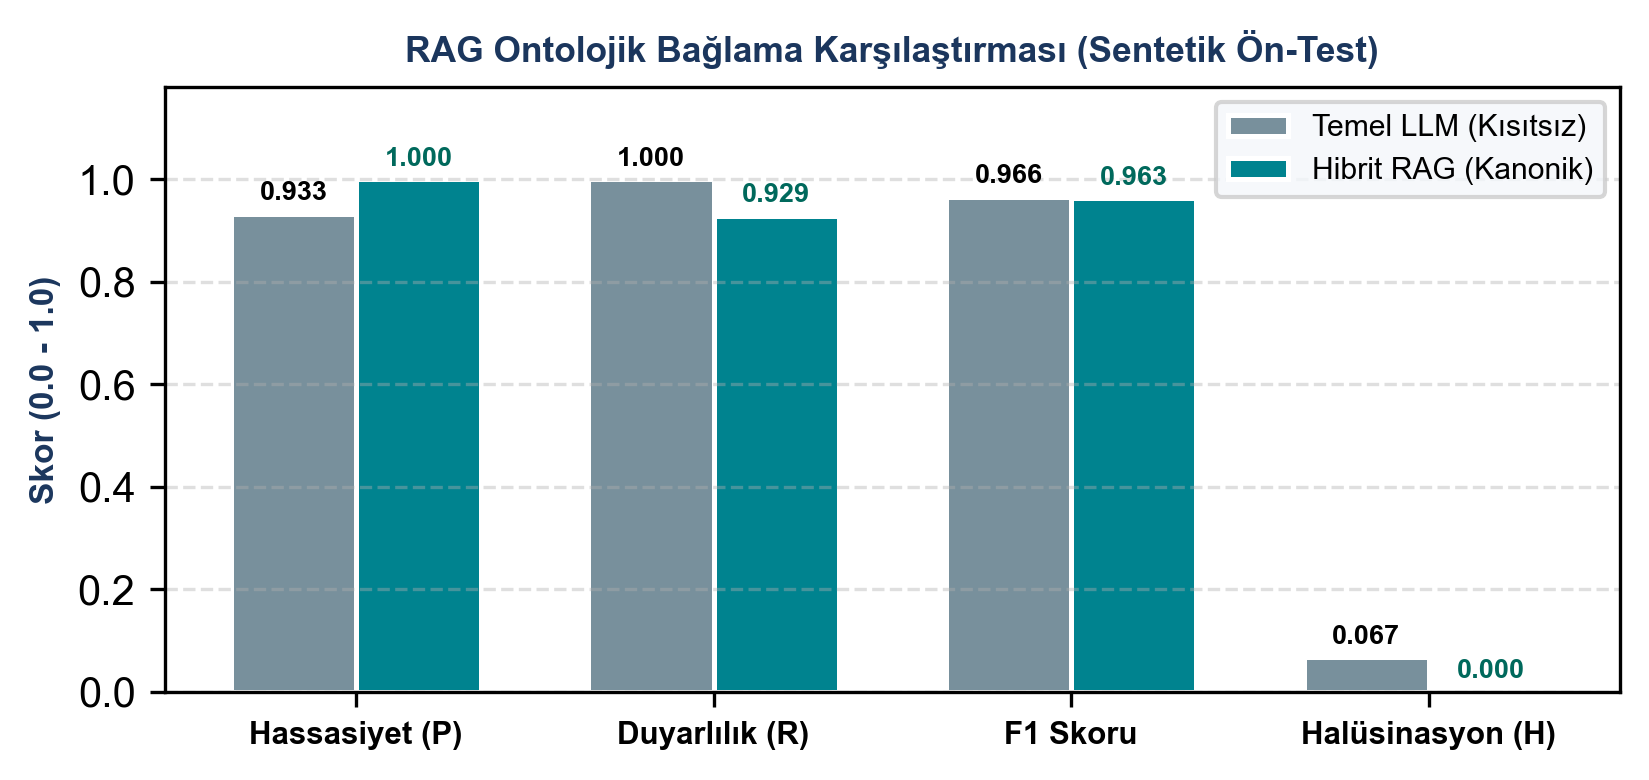
\includegraphics[width=\linewidth,height=6.0cm,keepaspectratio]{img/rag_performance_chart.png}
    \captionof{figure}{Şekil 6: Hibrit RAG Ontolojik Çıpalama (Grafik: Sentetik Ön-Test; Sondaj: 8 Klipte \%60.7).}

    \begin{itemize}
      \item \textbf{Kanonik Bilgi Tabanı:} 7 dikey sektörde kanonik terim tanımları ve Bloom taksonomisiyle ontolojik çıpalama.
      \item \textbf{Gerçek Kurumsal Sondaj (KVKK/İSG):} 8 uzun kurumsal konuşmada \%60.7 aday bağlamlama kesinliği (17/28 terim) ve 5 pedagojik önkoşul açığı tespit edilmiştir (grafikteki değerler sentetik ön-test ablasyonudur).
      \item \textbf{Önkoşul Grafı (DAG):} Derste atlanan pedagojik önkoşulların (\textit{missing prerequisites}) tespiti.
    \end{itemize}
  \end{block}

  \vskip-0.3ex
  \begin{block}{ÇAPRAZ KATMAN HATA YAYILIMI (ASR WER $\to$ LLM F1)}
    \centering
    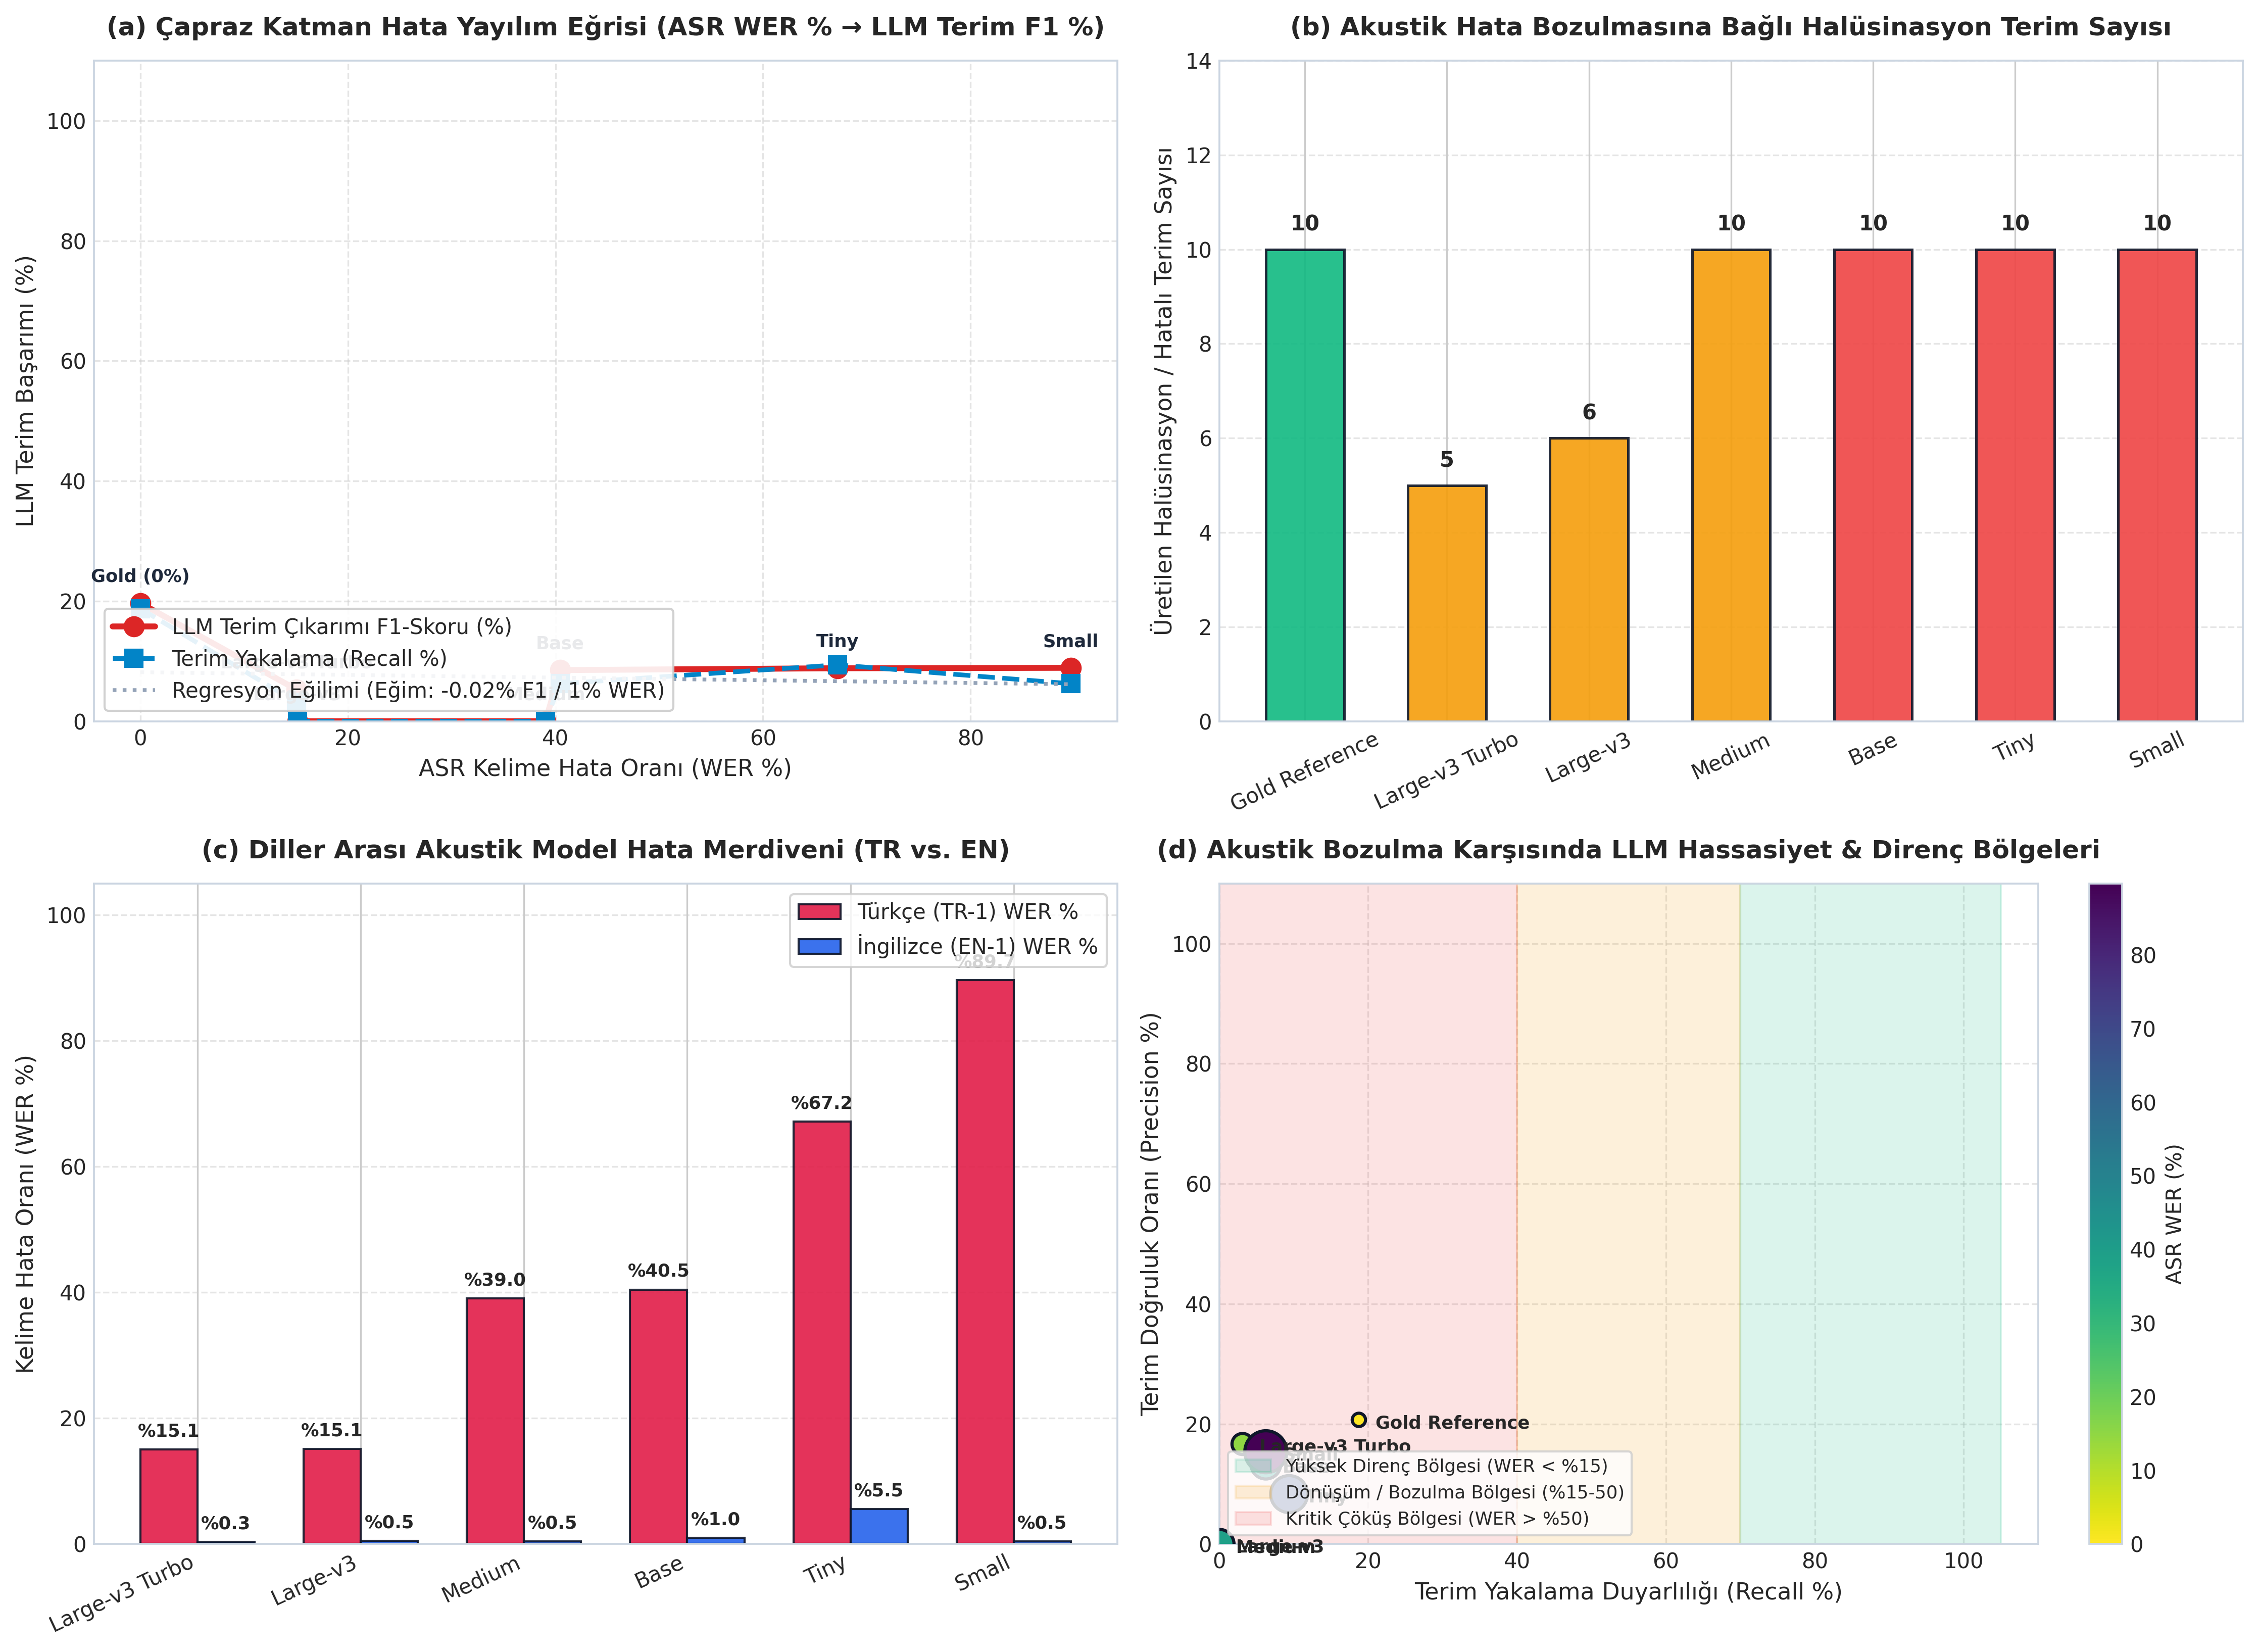
\includegraphics[width=\linewidth,height=5.8cm,keepaspectratio]{img/cross_layer_curve.png}
    \captionof{figure}{Şekil 7: Ampirik Hata Yayılım Eğrileri (A40, İş ID \texttt{33660}).}

    \begin{itemize}
      \item \textbf{7 ASR Basamağı (WER \%0 $\to$ \%89.7):} Gold referanstan Tiny/Small'a kadar aynı sesler taranmış ve 7B LLM ile kapalı 32 altın terimde test edilmiştir.
      \item \textbf{Duyarlılık Eğrileri:} $\Delta \text{WER} = +5\% \implies \Delta F_1 = -0.11\% \text{ (TR)} \text{ / } -1.23\% \text{ (EN)}$.
      \item \textbf{Tolerans Eşiği ($\text{WER} \le 15\%$):} Turbo ASR ile terim F1 korunurken, WER > \%40 seviyesinde halüsinasyon \%91.7'ye tırmanmaktadır.
    \end{itemize}
  \end{block}

\end{column}

% =========================================================================
% KOLON 4: Pedagojik DAG, Rekabetçi Matris, Sonuçlar ve Teşekkür
% =========================================================================
\separatorcolumn

\begin{column}{\colwidth}

  \begin{block}{TAM KORPUS (33 DERS) BİLGİ ÇİZGESİ (DAG) VE ÖNCÜL BOŞLUK ANALİZİ}
    \begin{itemize}
      \item \textbf{12 Disiplinde 33 Derslik Tam Hat:} Boğaziçi HPC A40 üzerinde tüm korpus 504.47 sn'de (~8.4 dk) işlenmiş; \textbf{118 teknik terim} ve 33 topolojik öğrenme rotası (DAG) çıkarılmıştır (İş ID \texttt{33600}).
      \item \textbf{19 Pedagojik Öncül Açığı Tespiti:} Temeli verilmeden ileri kavramlara geçilen noktalar DAG analiziyle bayraklanmıştır: KVKK'da (\texttt{TR-17}) \textbf{7 eksik öncül}, İSG'de (\texttt{TR-19/20}) \textbf{5'er eksik öncül} saptanmıştır.
      \item \textbf{CEFR B1 Uyumu:} Çıkarılan tanımların \textbf{\%57.6'sı} doğrudan B1 seviyesindedir.
    \end{itemize}

    \vskip0.2ex
    \centering
    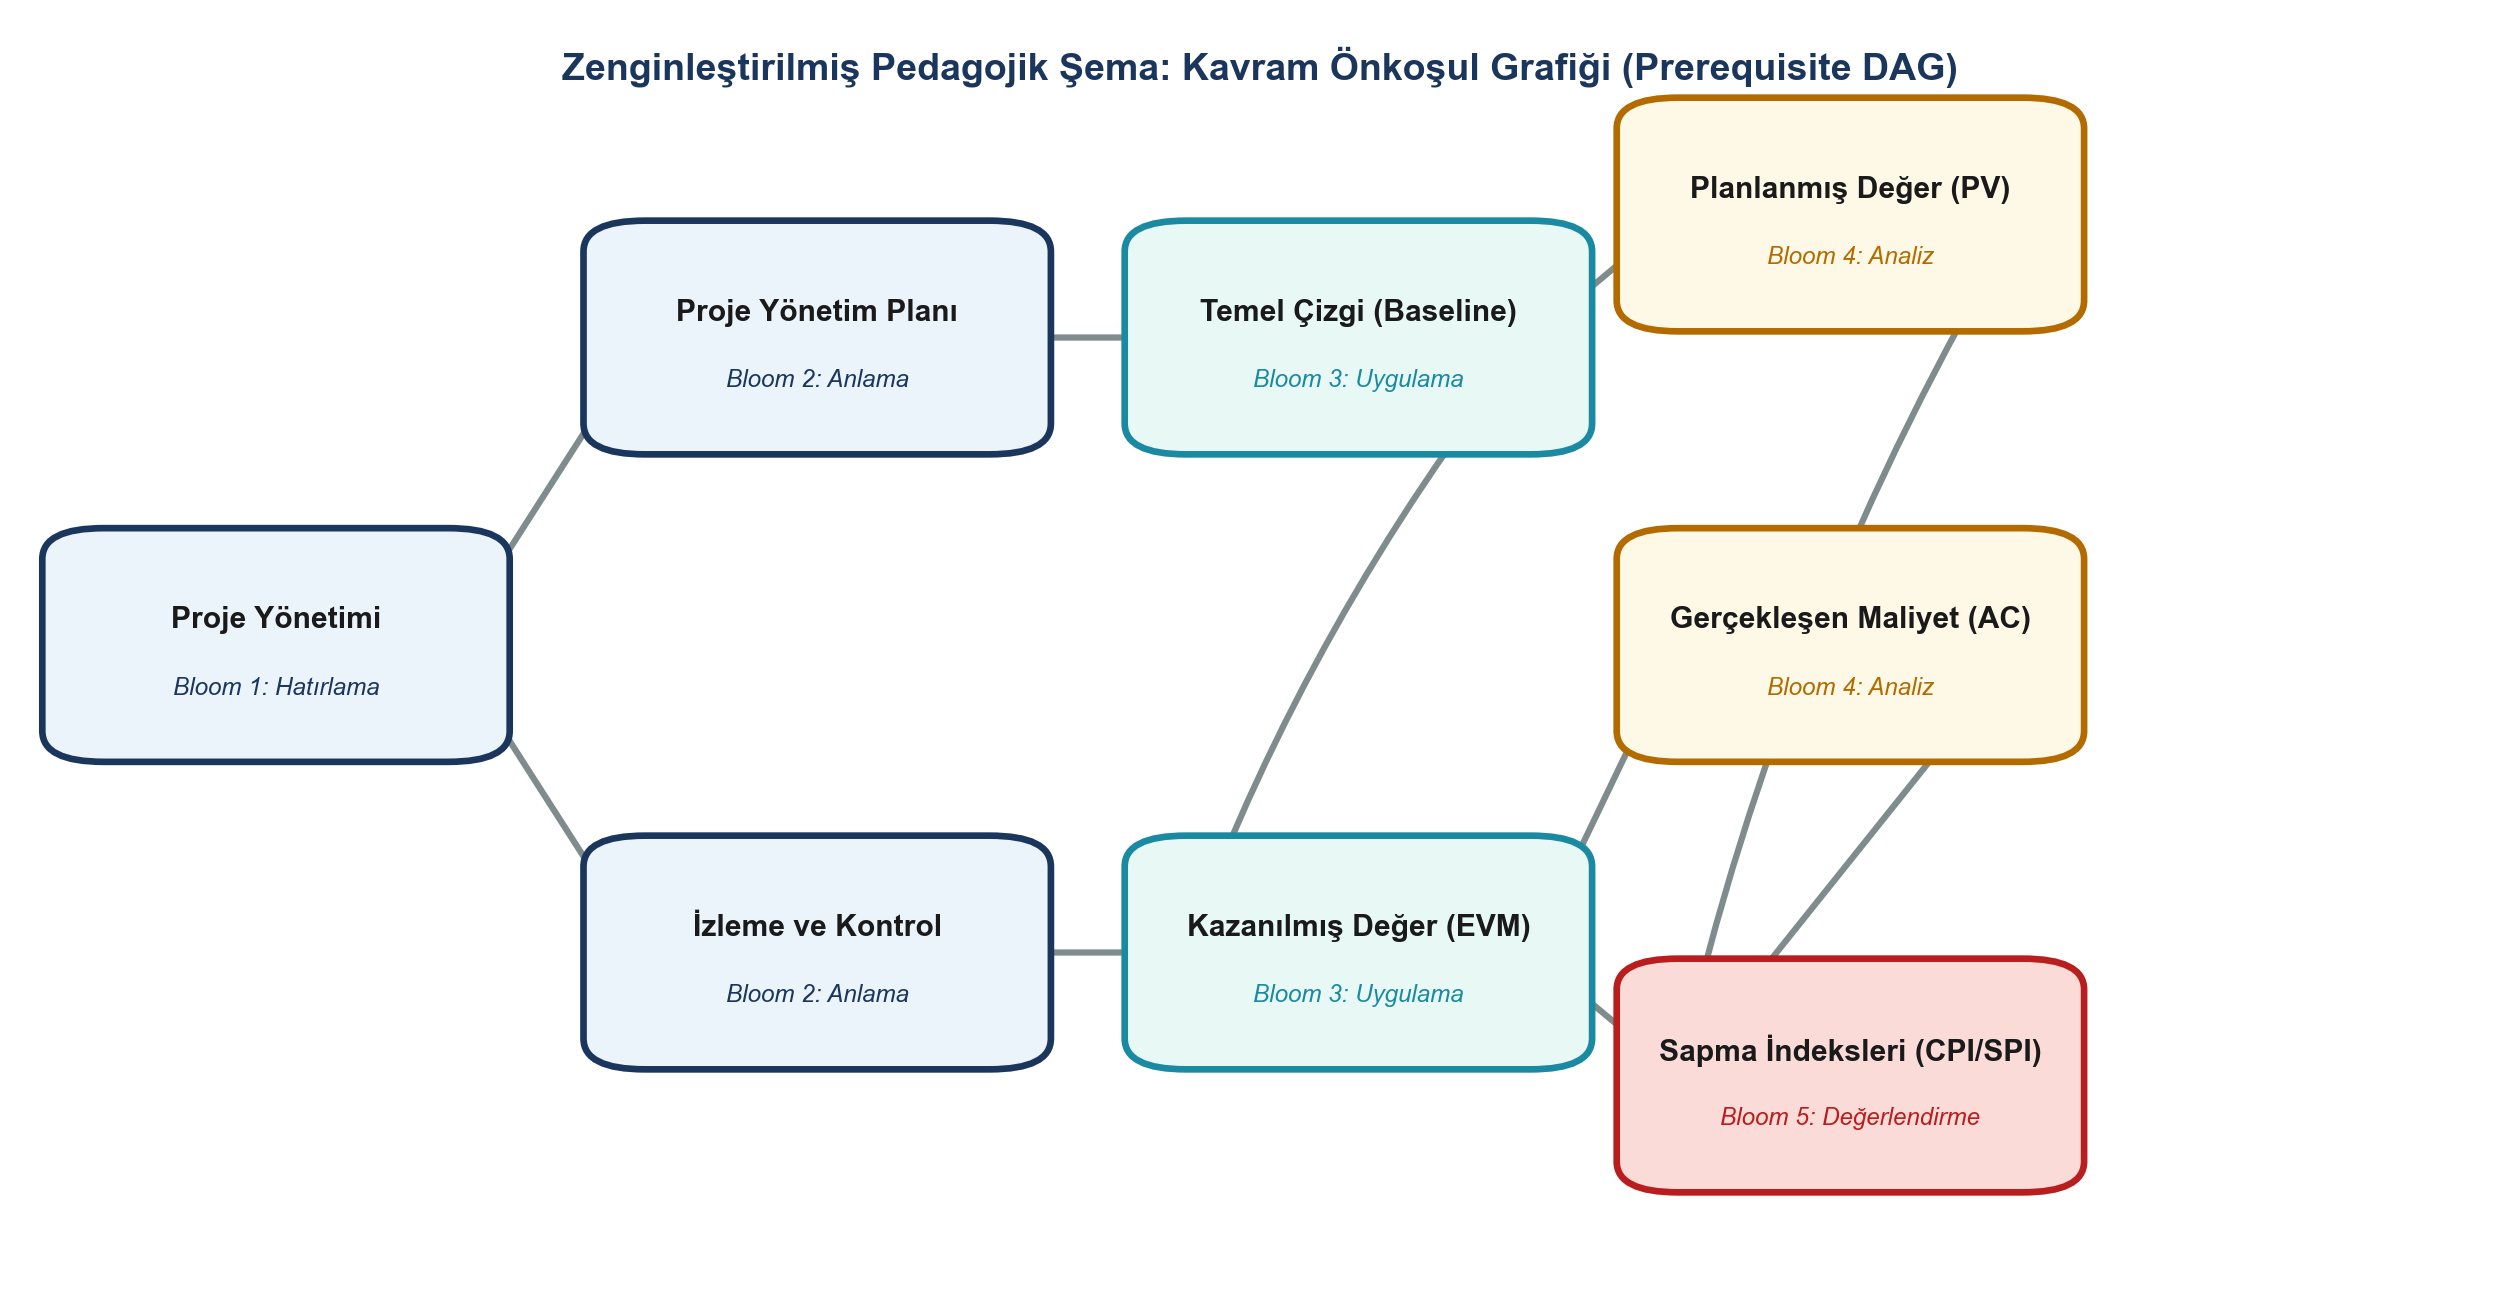
\includegraphics[width=0.94\linewidth,height=6.0cm,keepaspectratio]{img/concept_dag_graph.png}
    \captionof{figure}{Şekil 8: Pedagojik Kavram Önkoşul Grafiği ve Bloom Hiyerarşisi.}
  \end{block}

  \vskip-0.3ex
  \begin{block}{7 PLATFORMLU REKABETÇİ MATRİS}
    \small
    \begin{tabularx}{\linewidth}{>{\raggedright\arraybackslash}X c c c}
      \toprule
      \rowcolor{deepnavy}
      \textcolor{white}{\textbf{Özellik}} & \textcolor{white}{\textbf{EduTerm AI}} & \textcolor{white}{\textbf{Coursera/edX}} & \textcolor{white}{\textbf{Duolingo}} \\
      \midrule
      \textbf{ASR Terim Çıkarımı} & \textbf{Tam Otomatik} & Yok (Elle Altyazı) & Sınırlı \\
      \textbf{Kanonik RAG} & \textbf{Evet} & Hayır & Hayır \\
      \textbf{Önkoşul DAG} & \textbf{Evet (NetworkX)} & Statik Müfredat & Ağaç Bazlı \\
      \textbf{Uçta / Web GPU} & \textbf{Evet (WebGPU)} & Yalnızca Bulut & İstemci/API \\
      \textbf{CEFR B1 Sadeleştirme} & \textbf{Evet (Ateşman)} & Yok & A1--B2 Sabit \\
      \bottomrule
    \end{tabularx}
  \end{block}

  \vskip-0.3ex
  \begin{block}{NİHAİ SONUÇLAR VE GELECEK ÇALIŞMALAR}
    \begin{itemize}
      \item \textbf{Hibrit Dağıtım:} İstemcide hafif SRM/SLM (Whisper-Small + Qwen2.5-1.5B), sunucuda Whisper Large-v3 + EVREN H200 kümesi.
      \item \textbf{Gelecek Planı:} Moodle/Canvas LMS eklentisi ve dinamik öğrenci bilgi takip (\emph{Knowledge Tracing}) modeli.
    \end{itemize}
  \end{block}

  \vskip-0.3ex
  \begin{block}{KAYNAKÇA VE TEŞEKKÜR}
    \footnotesize
    \begin{enumerate}
      \item B. S. Bloom, ``The 2 sigma problem: 1-to-1 tutoring,'' \emph{Educ. Researcher}, 1984.
      \item A. Radford et al., ``Robust speech recognition via weak supervision,'' \emph{ICML}, 2023.
      \item J. Cohen, ``A coefficient of agreement for nominal scales,'' \emph{Educ. Psych. Meas.}, 1960.
    \end{enumerate}
    \vskip0.3ex
    \textbf{Teşekkür:} Boğaziçi Üniversitesi Lisans Bitirme Projesi (CMPE 492) kapsamında yürütülmüş; hesaplama desteği Boğaziçi Üniversitesi Bilgisayar Mühendisliği HPC Kümesi (NVIDIA A40 48GB), SSB / TÜBİTAK BİLGEM Millî EVREN YZ Platformu (H200) ve Tatilsepeti Ar-Ge Merkezi tarafından sağlanmıştır.
  \end{block}

\end{column}

\separatorcolumn
\end{columns}
\end{frame}

\end{document}
